\documentclass[border=10pt]{standalone}

\usepackage{tikz}
\usepackage{tikzsymbols}
\usetikzlibrary{calc,patterns,shapes.geometric}

\def\centerarc[#1](#2)(#3:#4:#5){\draw[#1] ($(#2)+({#5*cos(#3)},{#5*sin(#3)})$) arc (#3:#4:#5);}

\begin{document}
	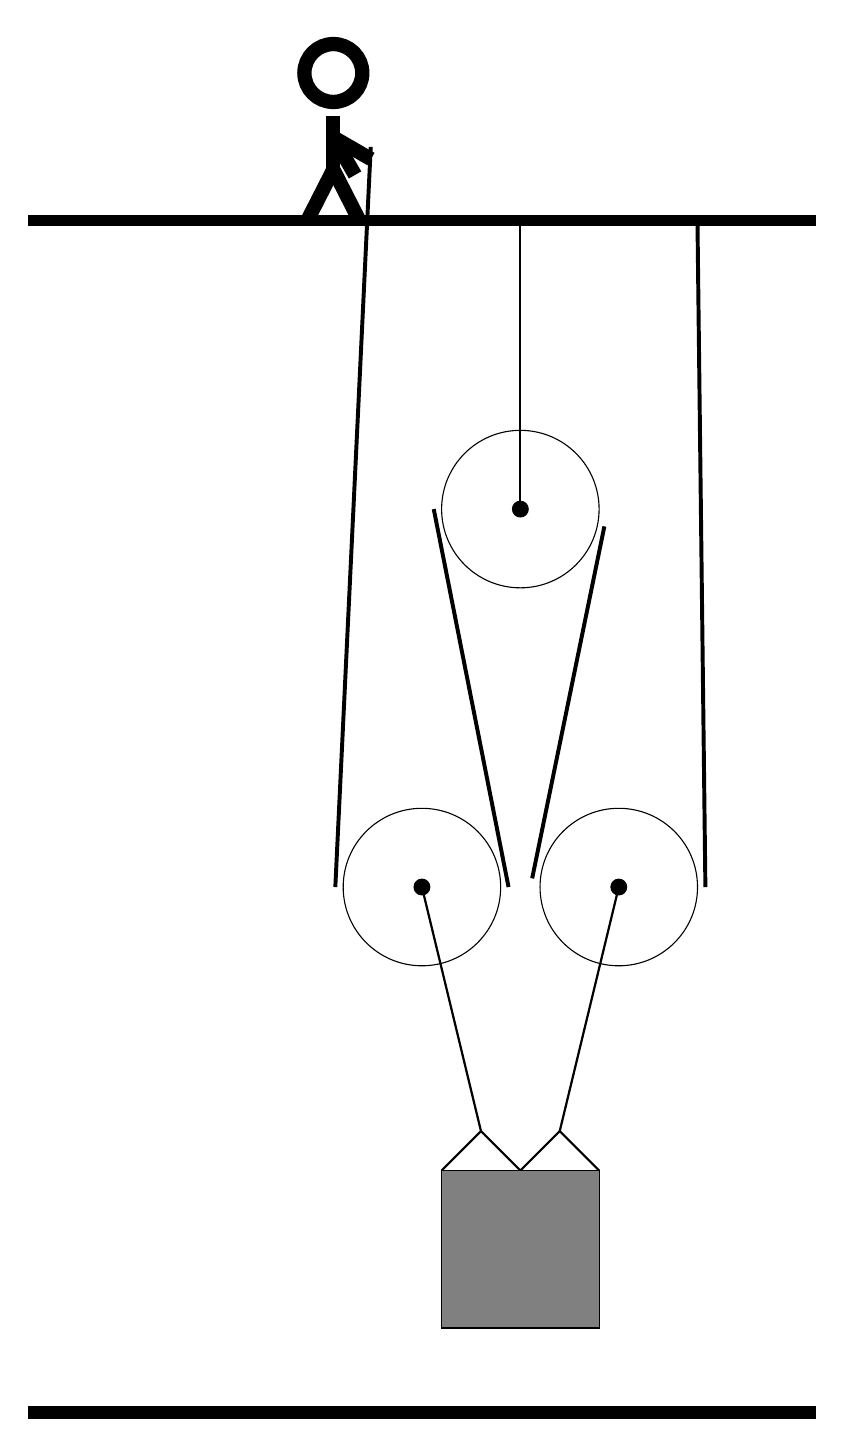
\begin{tikzpicture}
		%%%%% START %%%%%
		\draw[fill=black] (-4, 12) rectangle (6, 12.125);
		
		\draw (1, 3.6) circle (1);
		\draw[fill=black] (1, 3.6) circle (0.1);
		
		\draw (2.25, 8.4) circle (1);
		\draw[fill=black] (2.25, 8.4) circle (0.1);
		\draw[thick] (2.25, 8.4) -- (2.25, 12);
		
		\draw (3.5, 3.6) circle (1);
		\draw[fill=black] (3.5, 3.6) circle (0.1);
		
		\draw[thick] (3.5, 3.6) -- (2.75, 0.5);
		\draw[thick] (1, 3.6) -- (1.75, 0.5);
		\draw[thick]  (1.25, 0) -- (1.75, 0.5) -- (2.25, 0);
		\draw[thick]  (2.25, 0) -- (2.75, 0.5) -- (3.25, 0);
		\draw[fill=black!50] (1.25, 0) rectangle (3.25, -2);
		
		\draw[line width=0.5mm] (0.35, 13) --  (-0.1, 3.6);
		\centerarc[line width=0.5mm](1, 3.6)(180:360:1.1);
		\draw[line width=0.5mm] (2.1, 3.6) -- (1.15, 8.4);
		\centerarc[line width=0.5mm](2.25, 8.4)(-20:180:1.1);
		\draw[line width=0.5mm](3.317, 8.18) -- (2.4, 3.71);
		\centerarc[line width=0.5mm](3.5, 3.6)(160:360:1.1);
		\draw[line width=0.5mm](4.6, 3.6) -- (4.5, 12);
		
		\node at (-0.07, 13.2) {\Strichmaxerl[10][120][-30]};
		
		\draw[fill=black] (-4, -3) rectangle (6, -3.15);
		%%%%% END %%%%%
	\end{tikzpicture}
\end{document}